\documentclass[a4paper,12pt]{ctexart}
\usepackage{xeCJK}
\usepackage{booktabs}
\usepackage{enumerate}
\usepackage{graphicx}
\usepackage[normalem]{ulem}
\usepackage{amsmath}
\usepackage{amsfonts}
\usepackage{amssymb}
\usepackage{float}
\usepackage[hidelinks]{hyperref}
\usepackage[table,xcdraw]{xcolor}
\author{董晨阳 \thanks{学号2201211201} 李昭伦 \thanks{学号2201211203}}
\date{\today}
\title{风管模型基金运行报告}
\begin{document}
\maketitle
\tableofcontents
\section{风险偏好和目标设定}
作为2022年年底成立的新基金,本基金被动追踪一篮子股票的价值,持仓份额如表\ref{holdings} 所示。
\begin{table}[ht]
    \centering
    \begin{tabular}{lr}
        \toprule
        {} &    weights \\
        \midrule
        寒武纪  &  17.892709 \\
        浪潮信息 &  -1.756869 \\
        景嘉微  &  -5.328205 \\
        汤姆猫  &   8.344838 \\
        拓维信息 &   2.523862 \\
        中国电信 &   3.646449 \\
        中国移动 &   7.461063 \\
        科大讯飞 &  -9.595058 \\
        三六零  &  -7.383138 \\
        视觉中国 & -14.805651 \\
        \bottomrule
        \end{tabular}
	\caption{持仓权重}
	\label{holdings}
\end{table}

遵循一般私募基金运行惯例,本基金预警线设置为份额净值 0.8 元,止损线设置为份额净值 0.7 元。
触及预警线时,私募行业一般要求管理人及时减仓,直到净值重归预警线之上才能加仓。
触及止损线时,一般要求管理人无条件清仓,并将剩余的投资款返还客户。
双线作为一把“双刃剑”,一方面明确了安全边际,促使管理人谨慎投资并配置风控预案。另一方面,双线也加大了管理人在极端行情下的操作难度,大规模私募基金的减仓清盘行为甚至会加剧市场的波动。

本基金的业绩基准为沪深300 ETF。因而本基金的目标为在 300ETF 之上取得相对收益的同时,在四个月运行期间避免触及预警和清盘线。综上,本基金的风险偏好为每月最多亏损\(1-0.8^{1/4}\approx 0.05\),即每月净值下跌至多5\%。

本基金假定了股票交易成本为 0,期权价格采用二叉树公平定价。
\section{策略理由和面临的风险}
本基金持仓组合中的行业涉及金融、传统消费、新能源等行业,易受到整体经济运行环境的影响,当整体经济下行时,持仓组合中容易出现较大幅度的向下波动,因此我们选择通过购入反映整体股市波动的沪深300ETF进行对冲。我们采取 protective put 策略,即在持有股票的同时,每月月初在市场上购入适当的月末到期的、执行价格为95\% 的沪深300ETF 看跌期权。购入看跌期权。

每月具体下表所示单位基金的对冲期权数由两者的 \(\beta\) 计算得到。
计算结果如表 \ref{beta} 所示:
\begin{table}[H]
	\centering
	\begin{tabular}{ll}
		月份 & 1单位基金对冲期权数 \\\hline
		1月 & 0.4895       \\
		2月 & 0.5367       \\
		3月 & 0.5895       \\
		4月 & 0.8223       \\
	\end{tabular}
	\caption{\(\beta\) 变化}
	\label{beta}
\end{table}
我们的对冲策略面临的具体风险如下:
\begin{enumerate}
	\item 指数期权对冲效果不理想。
	      由于我国没有具体某只股票的期权,因此我们只能选择用指数期权对冲。存在指数与本基金基金相关性不强的风险,可能出现基金中标的资产下跌,指数上涨的情况,则会导致对冲效果不理想。
	\item 单位基金对冲数不足。
	      我们以月初计算得到的 \(\beta\) 值作为1单位基金的对冲期权数,实际上可能在月末行权时,我们计算得到的期权不能覆盖我们的损失,存在着对冲期权数不足的风险。
	\item 期权价格过高造成了较大的对冲成本。
	      我们每月初都会购入新的对冲期权,我们存在过度对冲的风险,由于期权的购买费用,给本基金的成本端造成了较大压力。
\end{enumerate}

\section{当前策略成果}

\begin{figure}[h]
    \centering
    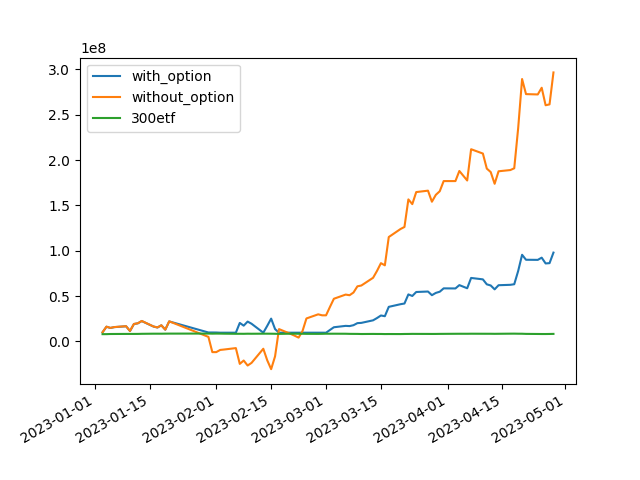
\includegraphics[width=0.8\linewidth]{./result.png}
    \caption{市值波动}
    \label{fig:300}
\end{figure}

图 \ref{fig:300} 展示了三种策略下持有的市值在2022年1-4月期间的波动状况。策略包括持有本基金并购买看跌期权、只持有本基金、只持有沪深300ETF这三种。结果由于持有市值大幅上涨超30倍,没有期权保护的反而收益率最高,但由于波动较大出现过持仓市值为负的margin call情形,而protective put策略则没有这样的风险。
\end{document}
